\documentclass[12pt]{article}
\usepackage{url, graphicx}
\usepackage{geometry}
\usepackage{amsmath}
\usepackage{fancyhdr}
\usepackage{nopageno}
\usepackage[usenames, dvipsnames]{color}

\pagestyle{fancy}

\title{\huge Lecture 9: Graph Algorithms: Depth First Search}
\author{}
\date{}
\pagestyle{fancy}
\fancyhf{}
\lhead{COMP 251 Winter 2018}
\rhead{Lecture 9}
\lfoot{$26^{th}$ Jan, 2018}
\rfoot{\copyright{}Yutong Yan}
\newcommand{\forceindent}{\leavevmode{\parindent=1em\indent}}
\begin{document}
\maketitle


\section{Depth First Search: Stack}
\renewcommand{\labelitemii}{$\circ$}
\renewcommand{\labelitemiii}{$\cdot$}
\renewcommand{\labelitemiii}{$\rightarrow$}
\renewcommand{\labelitemiv}{$\star$}
\begin{itemize}
\item Using a \textbf{Stack} (LIFO) data structure produces:\\
\underline{Depth First Search Algorithm}\\
Add (*, r) to a Stack\\
\forceindent \textbf{While} the Stack is non-empty\\
\forceindent \forceindent Remove the first arc (u, v) from the Stack\\
\forceindent \forceindent If v is unmarked \\
\forceindent \forceindent \forceindent Mark v\\
\forceindent \forceindent \forceindent Set $p(v) \leftarrow u$ \\ 
\forceindent \forceindent \forceindent For each arc(v,w)\\
\forceindent \forceindent \forceindent \forceindent Add (v, w) into the back of the Stack
\end{itemize}
\begin{center}
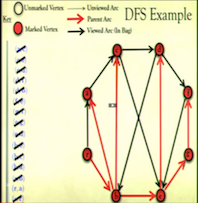
\includegraphics{lecture91}
\end{center}

\section{Depth First Search Trees}
\renewcommand{\labelitemii}{$\circ$}
\renewcommand{\labelitemiii}{$\cdot$}
\renewcommand{\labelitemiii}{$\rightarrow$}
\renewcommand{\labelitemiv}{$\star$}
\begin{itemize}
\item Recall, we proved that the search algorithm produces a search tree.\\
 \textbf{Theorem.} Let G be a connected, undirected graph. Then the predecessor edges form a tree rooted at r.
 \item However, the structure of the DFS tree is quite different from that of a BFS tree.
\end{itemize}

\section{Edge Structure in Undirected Graphs}
\renewcommand{\labelitemii}{$\circ$}
\renewcommand{\labelitemiii}{$\cdot$}
\renewcommand{\labelitemiii}{$\rightarrow$}
\renewcommand{\labelitemiv}{$\star$}
\begin{itemize}
\item Depth First Search partitions the edges of an undirected graph into two types:\\
\textbf{Tree Edges.} Predecessor edges in the DFS tree T.\\
\textbf{Back Edges.} Edges where one endpoint is an ancestor of the other endpoint in T.
\begin{center}
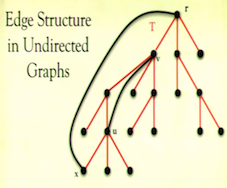
\includegraphics{lecture92}
\end{center}
\item When we perform a DFS, there is no crosses of the following type:\\
\textbf{Cross Edges.} Edges where neither endpoint is an ancestor of the other in T.
\begin{center}
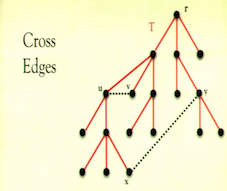
\includegraphics{lecture93}
\end{center}
\end{itemize}


\section{Depth First Search (Recursive Description)}
\renewcommand{\labelitemii}{$\circ$}
\renewcommand{\labelitemiii}{$\cdot$}
\renewcommand{\labelitemiii}{$\rightarrow$}
\renewcommand{\labelitemiv}{$\star$}
\begin{itemize}
\item The Depth First Search algorithm can be defined recursively:\\
\\
\forceindent \textbf{RecursiveDFS}(r)\\
\forceindent Mark r\\
\forceindent For each edge (r, v)\\
\forceindent \forceindent If v is unmarked\\
\forceindent \forceindent \forceindent Mark v\\
\forceindent \forceindent \forceindent For each arc (r, v)\\
\forceindent \forceindent \forceindent \forceindent Set $p(v) \leftarrow r$\\
\forceindent \forceindent \forceindent \forceindent \textbf{RecursiveDFS}(v)
\end{itemize}


\section{Depth First Search (Recursive Description)}
\renewcommand{\labelitemii}{$\circ$}
\renewcommand{\labelitemiii}{$\cdot$}
\renewcommand{\labelitemiii}{$\rightarrow$}
\renewcommand{\labelitemiv}{$\star$}
 \textbf{Theorem.} Let T be a DFS tree in an undirected graph G. Then, for every edge (u, v). wither u is an ancestor of v in T or v is an ancestor of u.\\
 \textbf{Proof.}
	\begin{itemize}
	\item Wlog assume u is marked before v.
	\item Consider the time u is marked during \textbf{RecursiveDFS}(u)
	\item In \textbf{RecursiveDFS}(u) the algorithm examines each arc incident to u.
	\end{itemize}
\underline{Case 1:} v is unmarked when \textbf{RecursiveDFS}(u) examines (u, v).
	\begin{itemize}
	\item The \textbf{RecursiveDFS}(u) sets $p(v) \leftarrow u$
		\begin{itemize}
		\item (u, v) is a tree edge.	
		\end{itemize}
	\end{itemize}
\underline{Case 2:} v is marked when \textbf{RecursiveDFS}(u) examines (u, v).
	\begin{itemize}
	\item But v was marked after u, so it was marked during \textbf{RecursiveDFS}(u)
	\item Thus, we have a series of vertices $\{u=w_0, w_1, ... , w_{l - 1}, w_l = v \}$ where $p(w_k) = w_{k - 1}$
		\begin{itemize}
		\item u is an ancestor of v in T.
		\item (u, v) is a back edge.
		\end{itemize}
	\end{itemize}
\begin{center}
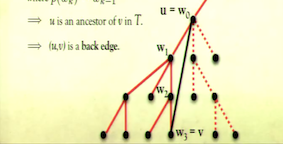
\includegraphics{lecture94}
\end{center}





\end{document}